\documentclass{beamer}
\usepackage{color}
\definecolor{greenish}{RGB}{152,204,112}
\definecolor{redish}{RGB}{244,158,196}


\usepackage{beamerthemeshadow}
\setbeamertemplate{navigation symbols}{}

\newcommand*{\LargerCdot}{\raisebox{-0.25ex}{\scalebox{3.0}{$\cdot$}}}

\begin{document}

\title{Active Learning}  
\author{Kacper Sokol}
\date{\today} 
\begin{frame}
\titlepage
\end{frame}




\begin{frame}
  \frametitle{Table of contents}
  \tableofcontents
\end{frame} 


\section{Concept of learning} 
  \subsection{Clustering}
  \begin{frame}%[plain]
    \frametitle{Find two clusters} 
    \begin{figure}
      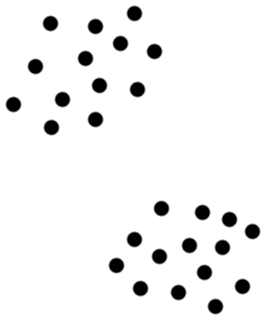
\includegraphics[scale=.5]{graphics/presentation/clusters1} 
    \end{figure}
  \end{frame}

  \begin{frame}%[plain]
    \frametitle{Find two clusters cont.} 
    \begin{figure}
      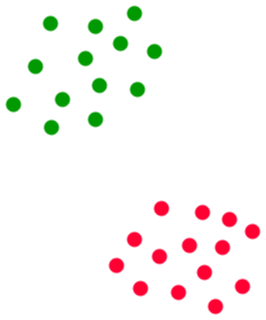
\includegraphics[scale=.5]{graphics/presentation/clusters1a} 
    \end{figure}
  \end{frame}

  \begin{frame}%[plain]
    \frametitle{Find two clusters cont.} 
    \begin{figure}
      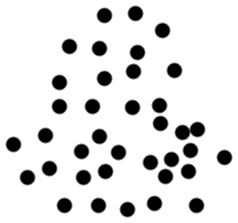
\includegraphics[scale=.5]{graphics/presentation/clusters2} 
    \end{figure}
  \end{frame}

  \begin{frame}%[plain]
    \frametitle{Find two clusters cont.} 
    \begin{figure}
      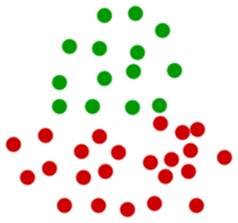
\includegraphics[scale=.5]{graphics/presentation/clusters2a} 
    \end{figure}
  \end{frame}

  \begin{frame}%[plain]
    \frametitle{Find two clusters cont.} 
    \begin{figure}
      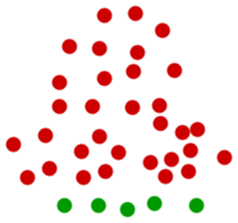
\includegraphics[scale=.5]{graphics/presentation/clusters2b} 
    \end{figure}
  \end{frame}

  \begin{frame}%[plain]
    \frametitle{Find two clusters cont.} 
    \begin{figure}
      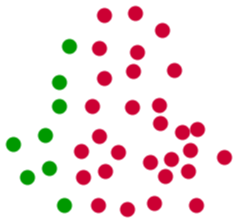
\includegraphics[scale=.5]{graphics/presentation/clusters2c} 
    \end{figure}
  \end{frame}

  \begin{frame}%[plain]
    \frametitle{Find two clusters cont.} 
    \begin{figure}
      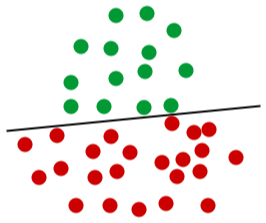
\includegraphics[scale=.5]{graphics/presentation/clusters2d} 
    \end{figure}
  \end{frame}

\subsection{The task}
  \begin{frame}
    \frametitle{Linear classifier}
    \begin{columns}
      \begin{column}{5cm}
        \begin{itemize}
          \item We are handling \textbf{binary classification}.
          \item The data are \textbf{linearly separable}.
          \item Therefore, our goal is to find two clouds of points separated by a straight line and make no error in separation.
        \end{itemize}
      \end{column}
      \begin{column}{5cm}
        \begin{figure}
          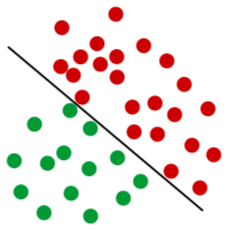
\includegraphics[scale=.4]{graphics/presentation/clusters2e} 
        \end{figure}
        \begin{itemize}
          \item green---a bike; red---a car
          \item x-axis---age of a person
          \item y-axis---distance form home to office/school
        \end{itemize}
      \end{column}
    \end{columns}
  \end{frame}

  \begin{frame}
    \frametitle{Linear classifier}
    \begin{block}{Theory of linear classifier}
      A linear classifier can be defined by a single vector $\mathbf{w} \in \mathbb{R}^N$, where dimension $N$ corresponds to number of parameters characterising our data---in this particular case $N=2$.
      $$
        \text{class}(\mathbf{x}) = \mathbf{w} \cdot \mathbf{x} - t \text{  ,  } \mathbf{x} \rightarrow \begin{cases} \textcolor{redish}{\LargerCdot} \text{ or } \textcolor{redish}{+} & \text{class}(\mathbf{x}) > 0 \\ \textcolor{greenish}{\LargerCdot} \text{ or } \textcolor{greenish}{-} & \text{class}(\mathbf{x}) < 0  \end{cases}
      $$
      In the above equation $t$ is arbitrarily chosen threshold.
    \end{block}
    \begin{block}{Evaluating the classifier---loss function}
      % ---is a value calculated for a given data points which
      \textit{Loss} describes how well given classifier fits the data; loss is positive if a point is classified correctly(the higher, the better), and it is negative if a point is classified incorrectly(the lower, the worse).
    \end{block}
  \end{frame}

  \begin{frame}
    \frametitle{Linear classifier, cont.}
    \begin{block}{Evaluating the classifier---loss function}
      % ---is a value calculated for a given data points which
      \textit{Loss} describes how well given classifier fits the data; loss is positive if a point is classified correctly(the higher, the better), and it is negative if a point is classified incorrectly(the lower, the worse).\\
      Exponential loss:
      $$
        L_{\text{exp}}(z) = \exp(-z) \text{  ,  } z(\mathbf{x}) = \text{label}(\mathbf{x}) * \text{class}(\mathbf{x}) \text{ ,}
      $$
      where $\text{label}(\mathbf{x})$ is the true class of datum point $\mathbf{x}$ i.e.\ $\textcolor{red}{+}$ or $\textcolor{green}{-}$.
    \end{block}
  \end{frame}

  \begin{frame}
    \frametitle{Supervised learning, cont.}
    In supervised learning we are given \emph{data points} together with their \emph{true class} and use this information to learn \emph{weight vector} $\mathbf{w}$.
    \begin{columns}
      \begin{column}{3cm}
        \begin{block}{Dataset---Spam}
          \begin{align*}
            (1,5)  & \rightarrow \textcolor{green}{\LargerCdot}\\
            (0,7)  & \rightarrow \textcolor{green}{\LargerCdot}\\
            (2,9)  & \rightarrow \textcolor{green}{\LargerCdot}\\
            (12,0) & \rightarrow \textcolor{red}{\LargerCdot}\\
            (8,3)  & \rightarrow \textcolor{red}{\LargerCdot}\\
            (13,1) & \rightarrow \textcolor{red}{\LargerCdot}
          \end{align*}
        \end{block}
      \end{column}
      \begin{column}{3cm}
        \begin{block}{Learn parameters}
          Use learning algorithm to learn weight vector $\mathbf{w}$ and class threshold $t$.\\
          ~\vspace*{.45cm}
          $$
            \mathbf{w} = (5,1)
          $$
          $$
            t = 33
          $$
        \end{block}
      \end{column}
      \begin{column}{3cm}
        \begin{block}{Classification}
          \begin{align*}
            -23 <0  & \rightarrow \textcolor{greenish}{\LargerCdot}\\
            -26  <0 & \rightarrow \textcolor{greenish}{\LargerCdot}\\
            -14  <0 & \rightarrow \textcolor{greenish}{\LargerCdot}\\
            27 >0 & \rightarrow \textcolor{redish}{\LargerCdot}\\
            10  >0 & \rightarrow \textcolor{redish}{\LargerCdot}\\
            33 >0 & \rightarrow \textcolor{redish}{\LargerCdot}
          \end{align*}
        \end{block}
      \end{column}
    \end{columns}
  \end{frame}

  \begin{frame}
    \frametitle{Supervised learning}
    Overall loss:
    \begin{multline*}
      \exp(-(\textcolor{green}{-} * -23)) + \exp(-(\textcolor{green}{-} * -26)) + \exp(-(\textcolor{green}{-} * -14)) +\\ \exp(-(\textcolor{red}{+} * 27)) + \exp(-(\textcolor{red}{+} * 10)) + \exp(-(\textcolor{red}{+} * 33)) =\\ 4.62315680937e-05 \text{ .}
    \end{multline*}
    \begin{columns}
      \begin{column}{5cm}
        \begin{block}{Dataset---Spam}
          \begin{align*}
            (1,5)  & \rightarrow \textcolor{green}{\LargerCdot} \text{~~~~} (12,0) & \rightarrow \textcolor{red}{\LargerCdot}\\
            (0,7)  & \rightarrow \textcolor{green}{\LargerCdot} \text{~~~~} (8,3)  & \rightarrow \textcolor{red}{\LargerCdot}\\
            (2,9)  & \rightarrow \textcolor{green}{\LargerCdot} \text{~~~~} (13,1) & \rightarrow \textcolor{red}{\LargerCdot}
          \end{align*}
        \end{block}
      \end{column}
      \begin{column}{5cm}
        \begin{block}{Classification}
          \begin{align*}
            -23 <0  & \rightarrow \textcolor{greenish}{\LargerCdot} \text{~~~} 27 >0 & \rightarrow \textcolor{redish}{\LargerCdot}\\
            -26  <0 & \rightarrow \textcolor{greenish}{\LargerCdot} \text{~~~} 10  >0 & \rightarrow \textcolor{redish}{\LargerCdot}\\
            -14  <0 & \rightarrow \textcolor{greenish}{\LargerCdot} \text{~~~} 33 >0 & \rightarrow \textcolor{redish}{\LargerCdot}
          \end{align*}
        \end{block}
      \end{column}
    \end{columns}
  \end{frame}

\subsection{Active learning}
  \begin{frame}
    \frametitle{Naive active learning}
  \end{frame}

  \begin{frame}
    \frametitle{Slightly better active learning}
  \end{frame}

  \begin{frame}
    \frametitle{Perfect active learning}
  \end{frame}


\section{Is it really exploration vs. exploitation?} 
\subsection{Multi-armed bandits as a workhorse}
  \begin{frame}
  \frametitle{MAB}
  \end{frame}

  \begin{frame}
  \frametitle{Ingredients of active learning}
  \end{frame}

  \begin{frame}
  \frametitle{Applying MAB to active learning}
  \end{frame}
\subsection{The experiment}
  \begin{frame}
  \frametitle{The dataset}
    \begin{figure}
      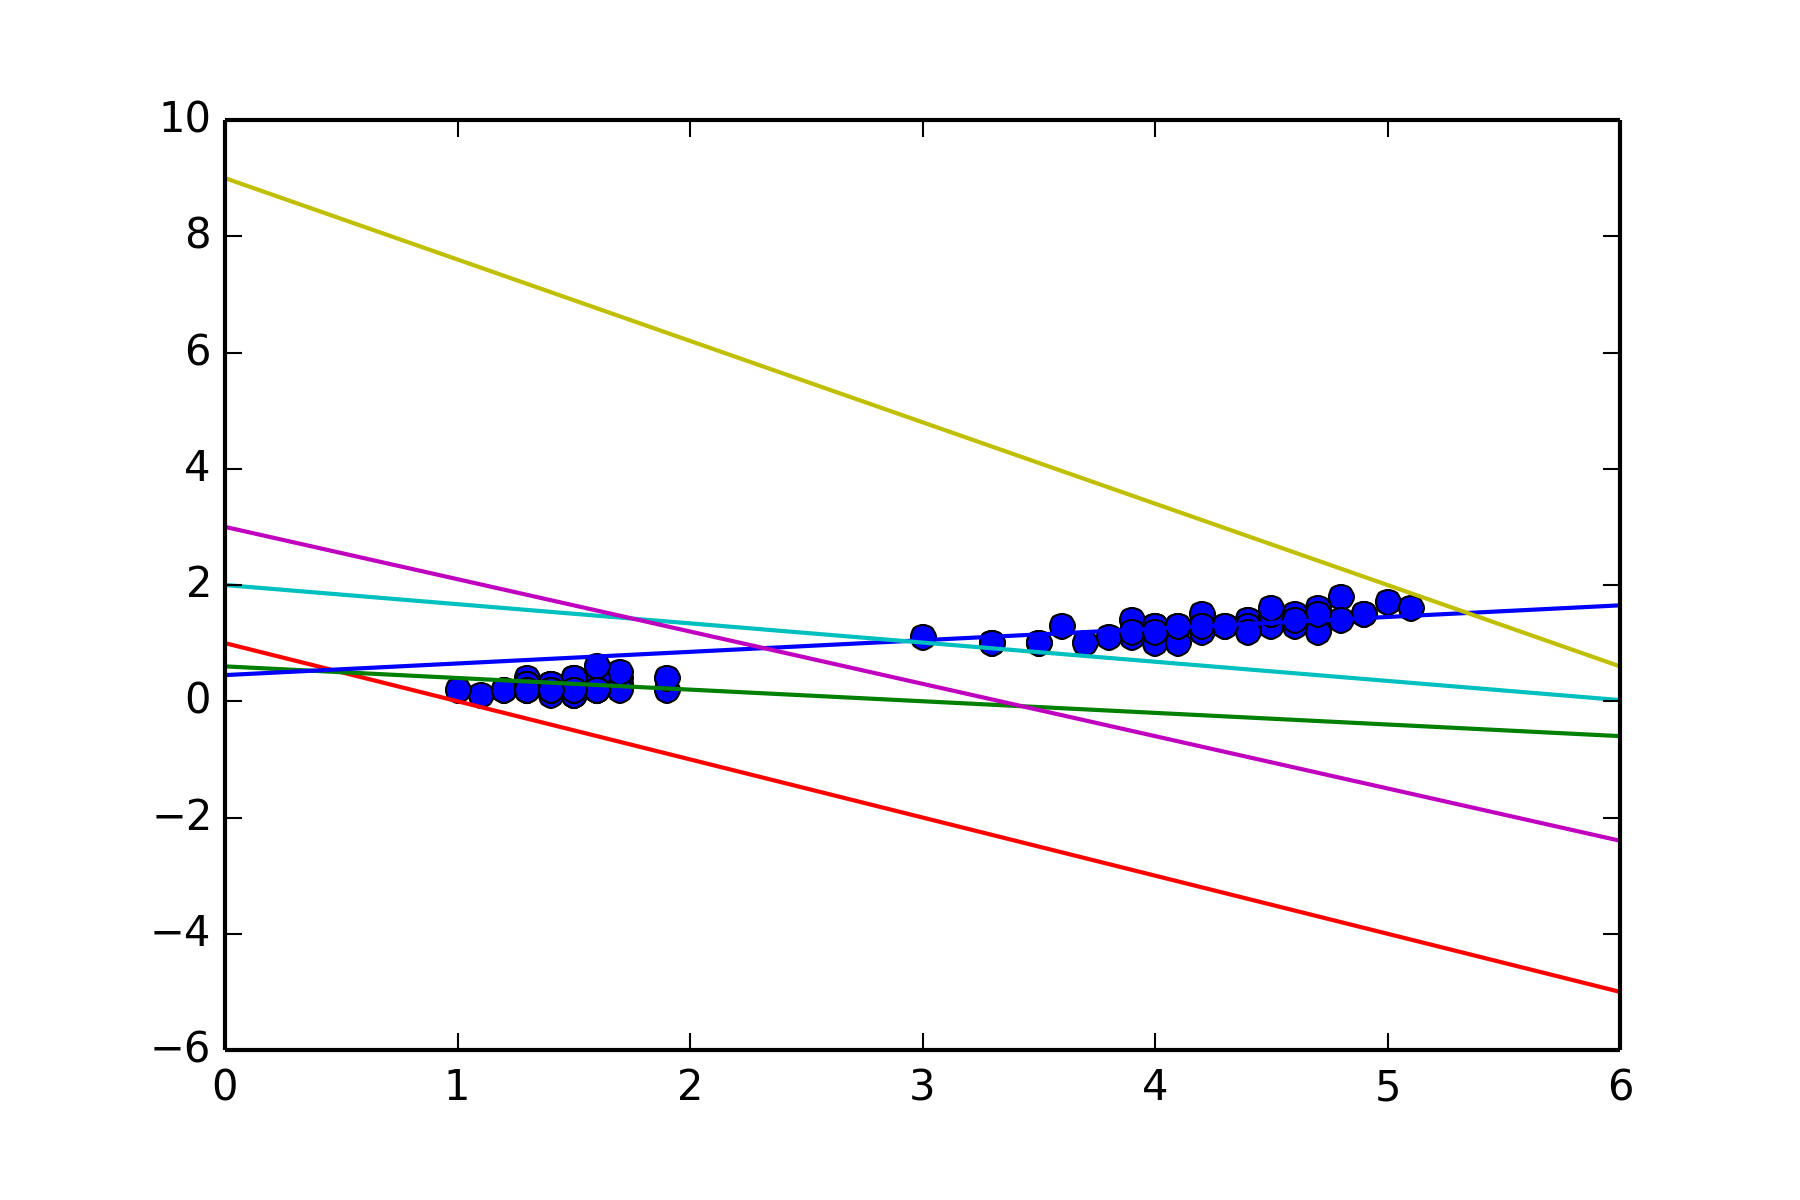
\includegraphics[scale=.7]{graphics/gypothesis} 
    \end{figure}
  \end{frame}
  \begin{frame}
  \frametitle{Arriving at optimal classifier}
    \begin{figure}
      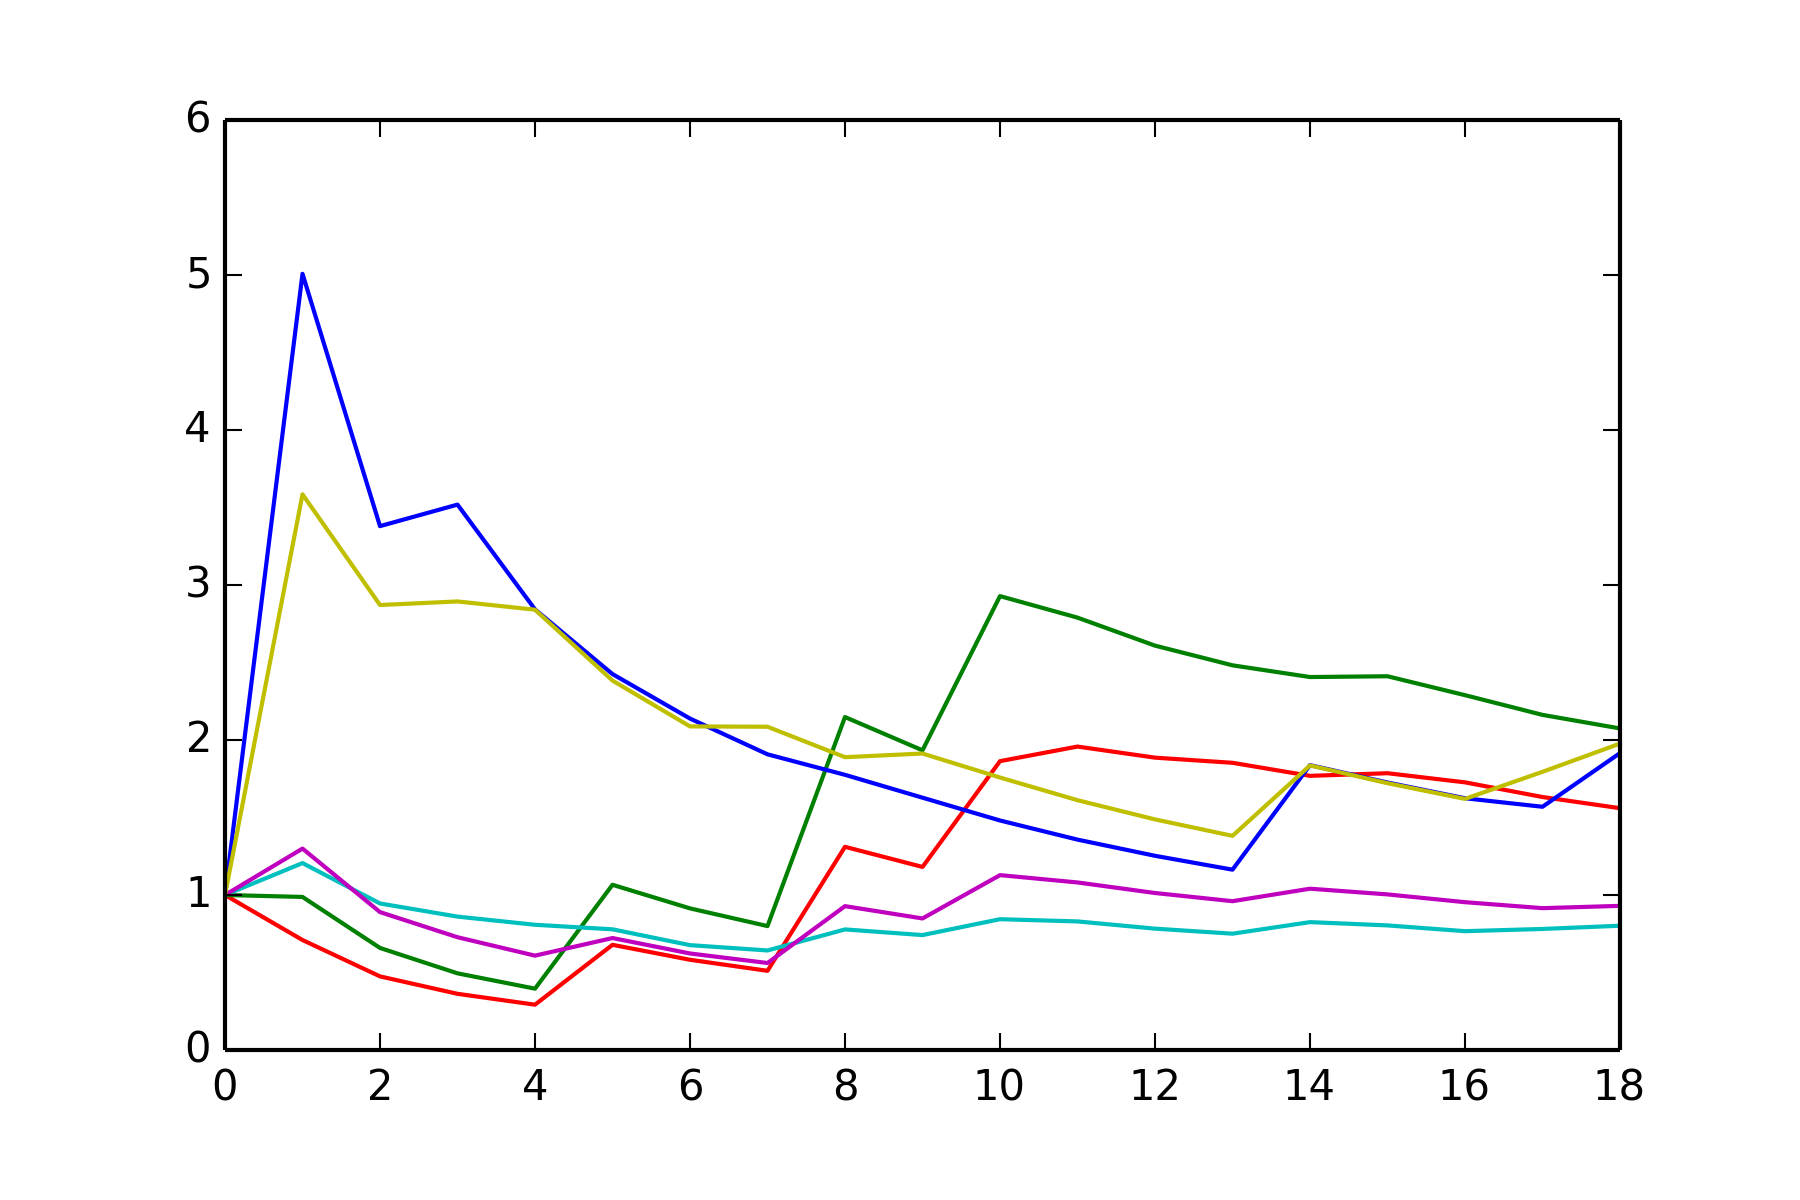
\includegraphics[scale=.7]{graphics/convergence15} 
    \end{figure}
  \end{frame}

\end{document}

%%%%%%%%%%%%%%%%%%%%%%%%%%%%%%%%%%%%%%%%%%%%%%%%%%%%%%%%%%%%%%%%%%%%%%%%%%%%%%%%
% \begin{block}{title of the bloc}
% bloc text
% \end{block}
%
% \begin{exampleblock}{title of the bloc}
% bloc text
% \end{exampleblock}
%
% \begin{alertblock}{title of the bloc}
% bloc text
% \end{alertblock}
% 
% 
% \pause 
% 
% \begin{itemize}
% \item<1-> subject 1
% \item<3-> subject 2
% \item<5-> subject 3
% \end{itemize}
% 
% 
% \begin{overprint}
% \includegraphics<2>{PIC1}
% \includegraphics<4>{PIC2}
% \includegraphics<6>{PIC3}
% \end{overprint}
%%%%%%%%%%%%%%%%%%%%%%%%%%%%%%%%%%%%%%%%%%%%%%%%%%%%%%%%%%%%%%%%%%%%%%%%%%%%%%%%
